\section{Разработка программного средства}

\subsection{Выбор языка программирования}
Robot Operating System (ROS) представляет собой широко используемую программную
платформу для разработки робототехнических систем, и одной из её ключевых
особенностей является то, что она написана на языке программирования C++. Этот
выбор не случаен: C++ считается стандартом индустрии благодаря своей высокой
производительности, гибкости и возможности работы на низком уровне с аппаратным
обеспечением. В контексте робототехники, где требуется быстрая обработка данных
с датчиков и управление механизмами в реальном времени, такие качества C++
становятся незаменимыми. Использование C++ в ROS позволяет разработчикам
создавать эффективные и масштабируемые решения для сложных задач, таких как
автономная навигация, обработка сигналов или взаимодействие с физическими
устройствами. Этот язык обеспечивает тонкий контроль над ресурсами системы, что
особенно важно для мобильных платформ с ограниченными вычислительными
мощностями. Кроме того, C++ обладает богатым набором библиотек и инструментов,
которые упрощают интеграцию ROS с другими технологиями, укрепляя его как
стандарта в индустрии робототехники.

Несмотря на все преимущества C++ как стандарта индустрии и основы для ROS, в
последние годы всё большее внимание в разработке программного обеспечения,
включая робототехнику, привлекает язык программирования Rust. В контексте ROS
уже появляются инициативы по интеграции Rust, что может дополнить или даже со
временем частично заменить C++, предлагая разработчикам более надёжный и удобный
инструмент для создания автономных систем, сохраняя при этом совместимость с
существующей экосистемой ROS.

Одним из ключевых преимуществ Rust является его способность обеспечивать
безопасность многозадачности. В отличие от C++, который требует дополнительных
усилий для безопасного выполнения параллельных операций, Rust изначально
предусматривает механизмы предотвращения гонок данных, что делает код более
надежным. Это особенно важно для системы навигации, где необходимо параллельно
обрабатывать данные с различных сенсоров и вычислять управляющие команды без
риска возникновения ошибок синхронизации.

Rust также предоставляет встроенные инструменты для работы с асинхронным
программированием, что позволяет эффективно организовать обработку данных в
реальном времени. Асинхронные операции позволяют системе собирать данные с
сенсоров, планировать маршрут и управлять моторами без блокировки основного
потока выполнения, что способствует повышению производительности и снижению
задержек.

Программная экосистема Rust активно развивается, и существует множество
библиотек, которые могут быть использованы для решения задач, связанных с
обработкой сенсорных данных, математическими расчетами и оптимизацией маршрутов.
Это позволяет разработчикам легко интегрировать необходимые инструменты и
сокращать время на разработку и тестирование системы. Также, благодаря хорошей
поддержке со стороны сообщества, Rust предоставляет разработчикам множество
ресурсов для быстрого решения возникающих вопросов.

Ключевым преимуществом Rust является его кроссплатформенность. Код, написанный
на этом языке, может быть скомпилирован для различных платформ, что делает Rust
отличным выбором для мобильных роботов, которые могут работать на разных типах
оборудования. Это позволяет без значительных усилий адаптировать систему под
разные архитектуры и аппаратные платформы.

Будущие улучшения системы могут включать в себя добавление новых сенсоров,
улучшение алгоритмов SLAM и маршрутизации, а также интеграцию с внешними
системами, такими как онлайн-карты или системы для прогнозирования дорожной
ситуации. Rust, благодаря своей гибкости и безопасному управлению памятью,
идеально подходит для такой работы, обеспечивая долгосрочную устойчивость и
развитие проекта.

Таким образом, проектирование программного обеспечения для системы мобильной
навигации с использованием сенсоров и алгоритмов SLAM требует тщательной
проработки архитектуры, выбора эффективных технологий и инструментов. Язык Rust
является отличным выбором для разработки таких систем, благодаря своим
преимуществам в безопасности, производительности и поддержке многозадачности,
что делает его идеальным для создания высоконадежных и высокопроизводительных
приложений для робототехники.

Robot Operating System (ROS) представляет собой широко используемую программную
платформу для разработки робототехнических систем, и одной из её ключевых
особенностей является то, что она написана на языке программирования C++. Этот
выбор не случаен: C++ считается стандартом индустрии благодаря своей высокой
производительности, гибкости и возможности работы на низком уровне с аппаратным
обеспечением. В контексте робототехники, где требуется быстрая обработка данных
с датчиков и управление механизмами в реальном времени, такие качества C++
становятся незаменимыми. Использование C++ в ROS позволяет разработчикам
создавать эффективные и масштабируемые решения для сложных задач, таких как
автономная навигация, обработка сигналов или взаимодействие с физическими
устройствами. Этот язык обеспечивает тонкий контроль над ресурсами системы, что
особенно важно для мобильных платформ с ограниченными вычислительными
мощностями. Кроме того, C++ обладает богатым набором библиотек и инструментов,
которые упрощают интеграцию ROS с другими технологиями, укрепляя его как
стандарта в индустрии робототехники.

Несмотря на все преимущества C++ как стандарта индустрии и основы для ROS, в
последние годы всё большее внимание в разработке программного обеспечения,
включая робототехнику, привлекает язык программирования Rust. В контексте ROS
уже появляются инициативы по интеграции Rust, что может дополнить или даже со
временем частично заменить C++, предлагая разработчикам более надёжный и удобный
инструмент для создания автономных систем, сохраняя при этом совместимость с
существующей экосистемой ROS.

Одним из ключевых преимуществ Rust является его способность обеспечивать
безопасность многозадачности. В отличие от C++, который требует дополнительных
усилий для безопасного выполнения параллельных операций, Rust изначально
предусматривает механизмы предотвращения гонок данных, что делает код более
надежным. Это особенно важно для системы навигации, где необходимо параллельно
обрабатывать данные с различных сенсоров и вычислять управляющие команды без
риска возникновения ошибок синхронизации.

Rust также предоставляет встроенные инструменты для работы с асинхронным
программированием, что позволяет эффективно организовать обработку данных в
реальном времени. Асинхронные операции позволяют системе собирать данные с
сенсоров, планировать маршрут и управлять моторами без блокировки основного
потока выполнения, что способствует повышению производительности и снижению
задержек.

Программная экосистема Rust активно развивается, и существует множество
библиотек, которые могут быть использованы для решения задач, связанных с
обработкой сенсорных данных, математическими расчетами и оптимизацией маршрутов.
Это позволяет разработчикам легко интегрировать необходимые инструменты и
сокращать время на разработку и тестирование системы. Также, благодаря хорошей
поддержке со стороны сообщества, Rust предоставляет разработчикам множество
ресурсов для быстрого решения возникающих вопросов.

Ключевым преимуществом Rust является его кроссплатформенность. Код, написанный
на этом языке, может быть скомпилирован для различных платформ, что делает Rust
отличным выбором для мобильных роботов, которые могут работать на разных типах
оборудования. Это позволяет без значительных усилий адаптировать систему под
разные архитектуры и аппаратные платформы.

Будущие улучшения системы могут включать в себя добавление новых сенсоров,
улучшение алгоритмов SLAM и маршрутизации, а также интеграцию с внешними
системами, такими как онлайн-карты или системы для прогнозирования дорожной
ситуации. Rust, благодаря своей гибкости и безопасному управлению памятью,
идеально подходит для такой работы, обеспечивая долгосрочную устойчивость и
развитие проекта.

Таким образом, проектирование программного обеспечения для системы мобильной
навигации с использованием сенсоров и алгоритмов SLAM требует тщательной
проработки архитектуры, выбора эффективных технологий и инструментов. Язык Rust
является отличным выбором для разработки таких систем, благодаря своим
преимуществам в безопасности, производительности и поддержке многозадачности,
что делает его идеальным для создания высоконадежных и высокопроизводительных
приложений для робототехники.

\subsection{Разработка цикла событий}

Программа спроектирована по принципу цикла событий, где мы обрабатываем
получаемые сообщения от системы.

В цикле прописаны обработчики каждого сообщения.
Виды сообщений:
\begin{itemize}
	\item сообщения от устройств периферии;
	\item сообщения от модуля навигации.
\end{itemize}

Каждый обработчик предполагает чтобы в нём не было трудоёмких вычислений, что
позволяет циклу событий непрерывно выполнятся вне зависимости от того какие
входные данные были получены.

% \subsection{Разработка модуля \todo{MotionEstimation}}

\subsection{Разработка UKF}
Фильтр описывается структурой:
\begin{lstlisting}
pub struct KallmanFilter<const N: usize, const K: usize, const S: usize> {
    pub state: SMatrix<f32, 1, N>,
    prior_state: Option<SMatrix<f32, 1, N>>,
    pub state_sigmas: Option<SMatrix<f32, S, N>>,
    pub state_noise: SMatrix<f32, N, N>,
    pub meas_sigmas: SMatrix<f32, S, K>,
    pub meas_noise: SMatrix<f32, K, K>,
    pub meas_covariance: Option<DMatrix<f32>>,
    pub inv_meas_covariance: Option<DMatrix<f32>>,
    pub covariance: SMatrix<f32, N, N>,
    prior_covariance: Option<SMatrix<f32, N, N>>,
    pub gain: Option<OMatrix<f32, Const<N>, Dyn>>,
    pub weights: SigmaWeights<S>,
}
\end{lstlisting}


Конструктор:
\begin{lstlisting}
pub fn new() -> Self {
     assert_eq!(sigma_order(N), S);

     let weights =
        sigma_points::estimate_merwe_weights::<N, S>(
            sigma_points::SigmaMetadata {
                alpha: 0.1,
                beta: 2.0,
                kappa: (N as f32 - 3.0),
            },
     );
     Self::with_weights(weights)
}

\end{lstlisting}

Расчёт весов сигма-точек выполняется в момент инициализации фильтра Калмана
следующим образом:
\begin{lstlisting}
pub fn estimate_merwe_weights<const N: usize, const S: usize>(
    metadata: SigmaMetadata,
) -> SigmaWeights<S> {
    assert!(S == sigma_order(N));
    let SigmaMetadata { alpha, beta, kappa } = metadata;
    let n = N as f32;
    let lambda = (alpha * alpha) * (n + kappa) - n;
    let c = 0.5 / (n + lambda);
    let mut w_m = vec![c; S];
    let mut w_c = vec![c; S];
    w_c[0] = lambda / (n + lambda) + (1.0 - alpha * alpha + beta);
    w_m[0] = lambda / (n + lambda);
    SigmaWeights {
        covariance: SVector::<f32, S>::from_vec(w_c).transpose(),
        mean: SVector::<f32, S>::from_vec(w_m).transpose(),
        sigma_order: S,
        metadata,
    }
}

\end{lstlisting}

Оценка значений сигма-точек выполняется по алгоритму:
\begin{lstlisting}
pub trait FnDistance<const N: usize>:
    Fn(SMatrixView<f32, 1, N>, SMatrixView<f32, 1, N>) -> SMatrix<f32, 1, N>
{/
}

pub fn estimate_merwe_sigmas<const S: usize, const N: usize, D>(
    state: SMatrixView<f32, 1, N>,
    covariance: SMatrixView<f32, N, N>,
    metadata: SigmaMetadata,
    distance_of: &D,
) -> Result<SMatrix<f32, S, N>, MathError>
where
    D: FnDistance<N>,
{
    let SigmaMetadata { alpha, kappa, .. } = metadata;
    let mean_estimations = {
        let state_size = N as f32;
        let lambda = alpha.powi(2) * (state_size + kappa) - state_size;
        let matrix = covariance.scale(lambda + state_size);
        let matrix = matrix.symmetric_part() + SMatrix::identity() * 0.0001;
        let Some(cholesky) = Cholesky::new(matrix) else {
            let dmatrix = DMatrix::from_iterator(
                matrix.nrows(),
                matrix.ncols(),
                matrix.iter().copied(),
            );
            return Err(MathError::CholeskyFailed(dmatrix));
        };
        cholesky.l()
    };
    let mut sigmas = SMatrix::<f32, S, N>::zeros();
    sigmas.row_mut(0).copy_from(&state);
    for i in 0..state.len() {
        let mean_estimation = mean_estimations.column(i).transpose();
        sigmas
            .row_mut(i + 1)
            .copy_from(&distance_of(state, (-1.0 * mean_estimation).as_view()));
        sigmas
            .row_mut(N + i + 1)
            .copy_from(&distance_of(state, (1.0 * mean_estimation).as_view()));
    }
    Ok(sigmas)
}

\end{lstlisting}

Для извлечения квадратного корня из матрицы ковариации $P$ используется
декомпозиция Холецкого. Операция декомпозиции определена только над
положительно\hyp{}определёнными матрицами. По определению, матрица ковариации всегда
положительно определена (элементами матрицы являются ковариации между
переменными). Но в процессе работы фильтра возможна ситуация, что матрица $P$
оказывается отрицательно-определённой.
Подобная ситуация возникает из-за:
\begin{itemize}
    \item накопления аппаратной вычислительной ошибки;
    \item особенностей способа обновления значений ковариаций в матриц;
    \item высокой сложности модели системы (более трёх переменных в векторе $X$).
\end{itemize}

В случае, если невозможно произвести декомпозицию по Холецкому,
предлагается сброс фильтра (см. подраздел \ref{subsec:motion_estimation}).

Ключевым этапом в работе UKF является реализация алгоритма преобразования  

\begin{lstlisting}
pub fn transform<T, F, const N: usize, const S: usize>(
    sigmas: &SMatrix<f32, S, N>,
    weights: &SigmaWeights<S>,
    noise_opt: Option<SMatrixView<f32, N, N>>,
    residual: &T,
    mean: &F,
) -> (SMatrix<f32, 1, N>, SMatrix<f32, N, N>)
where
    T: FnDistance<N>,
    F: FnMean<N, S>,
{
    let state = mean(weights.mean.as_view(), sigmas.as_view());

    let mut covariance = SMatrix::<f32, N, N>::zeros();

    for i in 0..S {
        let row = sigmas.row(i).clone_owned();

        let y = residual(row.as_view(), state.as_view());

        let mut outer = y.transpose() * y;
        outer.scale_mut(weights.covariance[i]);
        covariance += outer;
    }

    if let Some(noise) = noise_opt {
        //assert noise is diagonal matrix
        covariance += noise;
    }

    (state, covariance)
}
\end{lstlisting}

\subsection{Разработка модуля оценки состояния}
\label{subsec:motion_estimation}


Для удобства и повышения читаемости кода были объявлены типы данных для состояния и самого фильтра Калмана.
\begin{lstlisting}
pub type FilterState = ukf::FilterState<
    ACCEL_MODEL_STATE_SIZE,
    MEASUREMENT_SIZE,
    ACCELERATION_MODEL_SIGMA_ORDER
>;

pub type KallmanFilter = ukf::KallmanFilter<
    ACCEL_MODEL_STATE_SIZE,
    MEASUREMENT_SIZE,
    ACCELERATION_MODEL_SIGMA_ORDER,
>;
\end{lstlisting}

Для оценки модуль должен где-то хранить свои внутренние данные. Для этого была создана структура MotionEstimation. 

\begin{lstlisting}
pub struct MotionEstimation {
    pub config: MotionEstimationConfig,
    pub states: Vec<FilterState>,
    pub events: Vec<SensorEvent>,
    pub last_control_input: Option<ControlInput>,
    pub ukf_filter: KallmanFilter,
    pub imu_filter: Option<ImuFilter>,
}
\end{lstlisting}

При разработке модуля был применён событийно-риентированный подход к проектированию. Пересчёт предсказания позиции происходит только по прихождению сообщения от GPS, IMU и модуля сопоставления сканов.

\begin{lstlisting}
fn apply_event(
    &mut self,
    event: SensorEvent,
    observation_time: SystemTime,
) -> Result<(), LocalizationError> {
    let dt_secs = event
        .arrival_time()
        .duration_since(observation_time)
        .expect("Time goes in reverse order")
        .as_secs_f32()
        .max(0.001);

    let mut indices = Vec::<usize>::new();
    let mut meas_matrix = SVector::<f32, MEASUREMENT_SIZE>::zeros();

    match event {
        SensorEvent::MatchedPose(data) => {
            meas_matrix[SCAN_X] = data.coords.x;
            meas_matrix[SCAN_Y] = data.coords.y;
            meas_matrix[SCAN_THETA] = data.heading_rad;

            indices.push(SCAN_X);
            indices.push(SCAN_Y);
            indices.push(SCAN_THETA);

            self.imu_filter = None;
        }

	SensorEvent::Imu(data) => {
            let mut filter: ImuFilter =
                self.imu_filter.take().unwrap_or_else(|| {
                    ImuFilter::new(
                        self.config.epoch_duration_ms as f32 / 1000.0,
                        &self.get_estimated_state_unchecked(),
                        &self.config.noise,
                    )
                })
            filter.predict(dt_secs)?;
            filter.update(
                    dt_secs,
                    self.config.params.imu_filter,
                    &self.config.noise,
		    data
            )?;
	    return Ok(());
        }

        SensorEvent::GpsCoords(data) => {
            meas_matrix[GPS_X] = data.coords.x;
            meas_matrix[GPS_Y] = data.coords.y;

            indices.push(GPS_X);
            indices.push(GPS_Y);
        }
    }

    let transform = build_dyn_transform(&indices);

    let _ = self.predict(dt_secs)?;

    self.ukf_filter.update(
        &meas_matrix.transpose(),
        Some(transform),
        UpdateConfig {
            state_to_meas,
            mean_transform: meas_mean,
            meas_sub: meas_residual,
            state_sub: state_residual,
        },
    )?;

    Ok(())
}

\end{lstlisting}


Функции для преобразования сигма-точек
\begin{lstlisting}
fn meas_residual(
    m1: SMatrixView<f32, 1, MEASUREMENT_SIZE>,
    m2: SMatrixView<f32, 1, MEASUREMENT_SIZE>,
) -> SMatrix<f32, 1, MEASUREMENT_SIZE> {
    let mut m = m1 - m2;
    m[SCAN_THETA] = normalize_angle(m[SCAN_THETA]);
    m[IMU_THETA] = normalize_angle(m[IMU_THETA]);
    m
}

fn meas_mean(
    weights: SMatrixView<f32, 1, ACCELERATION_MODEL_SIGMA_ORDER>,
    sigmas: SMatrixView<f32, ACCELERATION_MODEL_SIGMA_ORDER, MEASUREMENT_SIZE>,
) -> SMatrix<f32, 1, MEASUREMENT_SIZE> {
    let column = sigmas.column(SCAN_THETA).transpose();

    let sum_sin = weights.dot(&column.map(f32::sin));
    let sum_cos = weights.dot(&column.map(f32::cos));

    let lidar_theta = f32::atan2(sum_sin, sum_cos);

    let column = sigmas.column(IMU_THETA).transpose();

    let sum_sin = weights.dot(&column.map(f32::sin));
    let sum_cos = weights.dot(&column.map(f32::cos));

    let imu_theta = f32::atan2(sum_sin, sum_cos);

    let x = weights.dot(&sigmas.column(SCAN_X).transpose());
    let y = weights.dot(&sigmas.column(SCAN_Y).transpose());

    let gps_x = weights.dot(&sigmas.column(GPS_X).transpose());
    let gps_y = weights.dot(&sigmas.column(GPS_Y).transpose());

    SMatrix::from_row_slice(&[
        x,
        y,
        lidar_theta,
        imu_theta,
        imu_v_theta,
        imu_a_x,
        imu_a_y,
        gps_x,
        gps_y,
        compass_theta,
    ])
}
\end{lstlisting}


% \subsection{Глобальный планировщик} % TODO
\subsection{Локальный планироващик}

Формирование минимальной скорости основывается
на тенденции к застреванию:
\begin{lstlisting}
let mut estimate_min_velocity = || -> Result<f32, LocalPlanError> {
    if rotation.abs() > config.stuck.rotation_tolerance
        || dist > *config.stuck.distance_tolerance
    {
        world.tracker.reset_stuck();
        return Ok(default_min_velocity);
    }
    let stuck_duration = world.tracker.detect_stuck();
    if stuck_duration < config.stuck.stuck_time_tolerance {
        return Ok(default_min_velocity);
    }
    if stuck_duration > config.stuck.max_stuck_time {
        return Err(LocalPlanError::StuckDetected);
    }

    let elapsed = stuck_duration;
    let max_elapsed = config.stuck.max_stuck_time;
    let v = config.robot.min_velocity
        + (config.robot.max_velocity - config.robot.min_velocity)
            * elapsed.as_secs_f32()
            / max_elapsed.as_secs_f32();

    if stuck_duration > config.stuck.stuck_time_force_backward {
        force_back_movement = true;
        Ok(v)
    } else {
        Ok(config.robot.max_velocity)
    }
};

\end{lstlisting}

Оценка максимальной скорости происходит по:
\begin{lstlisting}
let estimate_max_velocity = |state: &RobotState| -> f32 {
    let dist_to_goal =
        (world.target_pose.coords - state.position.coords).norm();
    let stop_time = dist_to_goal / config.robot.max_velocity;
    if stop_time <= limits.deceleration_time.as_secs_f32() {
        //slow deceleration
        let y = limits.deceleration_time.as_secs_f32();
        let base_pow = -y.log10() / y;
        let pow =
            base_pow * (limits.deceleration_time.as_secs_f32() - stop_time);
        let output = f32::exp(pow) * config.robot.max_velocity;
        output.clamp(config.robot.min_velocity, config.robot.max_velocity)
    } else if motion_time < limits.acceleration_time {
        //slow acceleration
        let x = motion_time.as_secs_f32();
        let a = x / limits.acceleration_time.as_secs_f32();
        f32::max(v_min, a.powi(3) * config.robot.max_velocity)
    } else {
        config.robot.max_velocity
    }
};
\end{lstlisting}

Оценка максимальной угловой скорости происходит (c задаваемой табличной функции $\omega_{max} = F(v)$):
\begin{lstlisting}
impl MovementOptimization {
    pub fn estimate_angular(&self, velocity: f32) -> f32 {
        let model = self.model.as_ref().unwrap();

        model
            .predict(&DenseMatrix::from_2d_vec(&vec![vec![velocity]]).unwrap())
            .unwrap()[0]
    }
}

let estimate_max_angular = move |state: &RobotState| -> f32 {
    let v_local = state.velocity.into_local(state.position.heading_rad);
    optimization
        .estimate_angular(v_local.translation.x)
        .clamp(0.0, max_angular)
};
\end{lstlisting}

Метрика выравнивания по углу в конечной точке: 
\begin{lstlisting}

pub fn target_alignment(&self, target_heading: f32) -> TrajectoryMetric {
    Box::new(move |trajectory| {
        let rotation = normalize_angle(
            trajectory.finish_state().position.heading_rad - target_heading,
        );
        let cost = rotation.abs() / f32::consts::FRAC_PI_2;
        Ok((MetricKind::TargetAlignment, MetricCost::new(cost)))
    })
}
\end{lstlisting}

Метрика кратчайшего пути
\begin{lstlisting}
pub fn shortest_path_metric(&self, goal: Point2<f32>) -> TrajectoryMetric {
    Box::new(move |trajectory| {
        let dist2 = (goal - trajectory.finish_state().position.coords)
            .norm_squared();

        Ok((MetricKind::ShortestPath, MetricCost::new(dist2)))
    })
}
\end{lstlisting}


Метрика коллизии:
\begin{lstlisting}
pub fn collision_metrics(
    &self,
    obstacles: &'a DynamicObstacles,
    map_chunk: &'a MapChunk,
) -> TrajectoryMetric {
    let robot = self.robot;
    let config = self.planner_config;
    Box::new(move |trajectory| {
        for state in trajectory.states.iter() {
            let state_shape = robot.build_shape(
                map_chunk.resolution,
                config.collision_distance,
                &(*state).into(),
            );
            if has_dynamic_collision(&state_shape, obstacles)
                || has_static_collision(&state_shape, map_chunk)
            {
                //collisions are not acceptable
                return Err(MetricError::Unreacheable);
            }
        }
        Ok((MetricKind::Collision, MetricCost::ZERO))
    })
}
\end{lstlisting}

Для расчёта метрики удалённости от коллизий в позиции можно заранее просчитать
расстояние до ближайшего препятствия в каждой точке, что превратит
вычислительную задачу в поисковую.



Метрика удалённости от коллизий:
\begin{lstlisting}
fn collision_map_metric(
    &'a self,
    map: &'a DistanceGrid,
    maybe_obstacles: Option<&'a DynamicObstacles>,
) -> TrajectoryMetric<'a> {
    Box::new(move |trajectory| {
        let state = trajectory.finish_state();
        let mut min_dist = f32::MAX;
        let coords = state.position.coords;
        let dist_cost = map.index_distance(&coords);
        if dist_cost.is_reacheable() {
            let dist = map.resolution.to_metres(dist_cost.as_f32());
            min_dist = f32::min(min_dist, dist);
        }
        if let Some(obstacles) = maybe_obstacles {
            let obstacle = obstacles.closest(&coords);
            let dist_to_dynamic_obstacle = (obstacle - coords).norm();
            min_dist = f32::min(min_dist, dist_to_dynamic_obstacle);
        }
        Ok((
            MetricKind::CollisionDistance,
            MetricCost::new(1.0 / min_dist),
        ))
    })
}
\end{lstlisting}

Метрика близости траектории к глобальному маршруту:
\begin{lstlisting}
fn distance_map_metric(
    &'a self,
    distance_grid: &'a DistanceGrid,
) -> TrajectoryMetric<'a> {
    Box::new(move |trajectory| {
        let states = &trajectory.states;
        let mut distance_cost = 0.0;
        for state in states.iter() {
            let world_point = state.position.coords;
            let distance = distance_grid.index_distance(&world_point);
            if distance.is_unreacheable() {
                return Err(MetricError::Unreacheable);
            }
            distance_cost += distance.as_f32();
        }
        Ok((MetricsKind::GlobalPath, MetricCost::new(distance_cost)))
    })
}
\end{lstlisting}

% \subsection{Разработка модуля \todo{BigMap}}

% \begin{figure}[h]
% \centering
% 	\fbox{
% 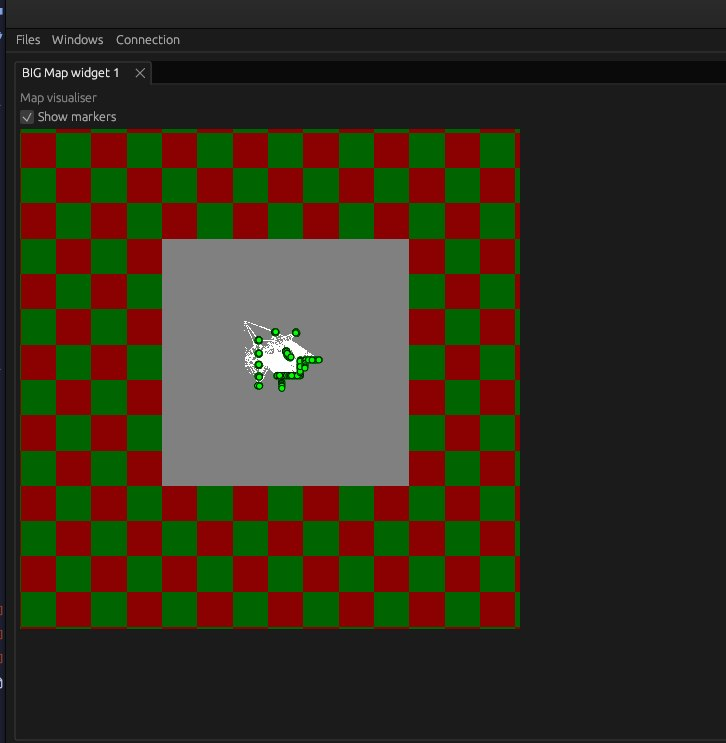
\includegraphics[width=14cm]{BIG_MAP}
% }
% \caption{Отображение BigMap в программе отладки}
% \end{figure}


% \subsection{Разработка модуля \todo{ScanMatching}}
\subsection{SLAM}
Задача построения карты заключается в добавлении новых данных поступающих с
датчиков на уже построенную карту. В качестве входных данных у нас данные с
лидара с позицией в которых они были произведены, а так-же карта на которую
происходит наложение скана.

В качестве алгоритма наложения был выбран алгоритм ICP (Iterative closest
point), который был разработан с использованием наработок в KISS ICP. Алгоритм
заключается в итеративном приближении наложения скана к карте.

Код наложение снимков лидара c облаком точек:
\begin{lstlisting}
pub fn match_points_cloud_with_kdtree(
    config: &IcpConfig,
    mut source: PointCloud,
    target: &KdTree,
) -> (IsometryMatrix2<f32>, PointCloud) {
    let initial_source = source.clone();

    let mut prev_error = 0.0;
    let mut _iter_count = 0;

    for _i in 0..config.max_iterations {
        _iter_count = _i;

        let (new_source_points, new_target_points) = nearest_neighboor_kdtree(
            &source,
            target,
            config.max_distance_for_nn_matching,
        );

        //source points are unknown
        //therefore no assumption about transform must be done
        if new_source_points.is_empty() {
            return (IsometryMatrix2::identity(), source);
        }

        let (trans, rot, error) =
            best_fit_transform(&new_source_points, &new_target_points);

        for point in source.iter_mut() {
            *point = Point2::from(trans + rot * point.coords);
        }

        if (error - prev_error).abs() < config.delta_error_stop
            || error.abs() < config.min_error_stop
        {
            break;
        }

        prev_error = error;
    }

    let transformation = best_fit_transform(&initial_source, &source);

    (
        IsometryMatrix2::from_parts(
            transformation.0.into(),
            Rotation2::from_matrix(&transformation.1),
        ),
        source,
    )
}
\end{lstlisting}

\subsection{Отправка команд на шасси}
На гусеничном шасси установлены два электромотора. Драйвера электромоторов упровляются по UART. Для корректного управления ходовой был написан слой, который транслирует команды модуля навигации в команды моторов и отправляет их по UART.

\begin{lstlisting}
#[tokio::main]
async fn main() {
    env_logger::builder().init();
    let term_flag = Arc::new(AtomicBool::new(false));

    for sig in signal_hook::consts::TERM_SIGNALS {
        signal_hook::flag::register_conditional_shutdown(
            *sig,
            42,
            Arc::clone(&term_flag),
        )
        .expect("Failed to set conditional shutdown");
        signal_hook::flag::register(*sig, Arc::clone(&term_flag))
            .expect("Failed to set default sig handler");
    }

    #[cfg(not(feature = "async"))]
    let driver = driver();
    #[cfg(feature = "async")]
    let driver = driver().await;

    let config = config();
    let odometry_timeout_ms =
        parse_env!("ODOMETRY_TIMEOUT", u64).unwrap_or(200);

    let dispatcher = MotorDispatcher::new(
        (&term_flag).into(),
        driver,
        Duration::from_millis(odometry_timeout_ms),
    );
    let _ = servers::priority::run(dispatcher, config).await;

    debug!("Exiting after termination signal");
}
\end{lstlisting}

В примере кода выше происходит конфигурация каналов связи с модулем навигации и моторами. 
Так же выставляется время отключения моторов при отсутсвии потока команд. Это сделано для безопасности, чтобы исключить ситуацию продолжения езды платформы при зависании программы модуля навигации.

Так как на одноплатном компьютере есть операционная система Linux, то взаимодействие с моторами по UART сводится к записи в файл.

\begin{lstlisting}
#[cfg(feature = "serial")]
fn driver() -> impl MotorDriver {
    use drivers::SerialMotor;

    let config = motor_config();

    let device_path = parse_env!("MOTOR_DEVICE", String)
        .unwrap_or("/dev/ttyUSB0".to_string());
    info!("Motor device: {device_path}");
    SerialMotor::new(device_path, config).expect("Failed to create serial port")
}
\end{lstlisting}

\subsection{Построение маршрута по карте}


На гусеничном шасси установлены два электромотора. Драйвера электромоторов упровляются по UART. Для корректного управления ходовой был написан слой, который транслирует команды модуля навигации в команды моторов и отправляет их по UART.

